\documentclass{"../../res/univ-projet"}
\usepackage[utf8]{inputenc}
\usepackage[T1]{fontenc}
\usepackage[francais]{babel}
\usepackage{colortbl}
\usepackage{algorithm}
\usepackage{algorithmic}


\logo{../../res/logo_univ.png}
\title{Architecture Logicielle}
\author{\bsc{Picard} Damien}
\projet{M1SSI}
\projdesc{Projet de génération d'OTP}
\filiere{M1SSI}
\version{1.0}
\relecteur{\bsc{Adegoloye} Tayewo John Yves}
\signataire{\bsc{Bardet} Magali}
\date{Décembre 2013}

\histentry{1.0}{01/12/2013}{Version relue et corrigée}
\histentry{0.1}{21/11/2013}{Premier jet}


\begin{document}
\maketitle
%-------------------------------------------------------------------------------
\section{Objet}
Ce document à pour but de préciser les détails techniques du logiciel final.

\section{Documents de référence}
\subsection{Documents de spécifications}
\begin{tabular}{p{1,5cm}>{\raggedright\arraybackslash}p{13cm}}
    {[ANS10]} & {ANSSI. Référentiel général de sécurité. \href{http://www.ssi.gouv.fr/fr/reglementation-ssi/referentiel-general-de-securite}{http://www.ssi.gouv.fr/fr/reglementation-ssi/referentiel-general-de-securite}, 2010.}
    \tabularnewline
    \\
    {[MvOV97]} & {Alfred J. Menezes, Paul C. van Oorschot, and Scott A. Vanstone. Handbook of applied cryptography. CRC Press Series on Discrete Mathematics and its Applications. CRC Press, Boca Raton, FL, 1997. With a foreword by Ronald L.Rivest.}
    \tabularnewline
    \\
    {[RFC98]} & {A One-Time Password System. \href{http://tools.ietf.org/html/rfc2289}{http://tools.ietf.org/html/rfc2289}, 1998.}
    \tabularnewline
    \\
    {[RFC05]} & {HOTP:An HMAC-Based One-Time Password Algorithm \href{http://tools.ietf.org/html/rfc4226}{http://tools.ietf.org/html/rfc4226}, 2005.}
    \tabularnewline
    \\
    {[RFC06]} & {Generic Message Exchange Authentication for the Securer Shell Protocol (SSH).\href{http://tools.ietf.org/html/rfc4256}{http://tools.ietf.org/html/rfc4256}, 2006.}
    \tabularnewline
    \\
    {[RFC07]} & {The EAP Protected One-Time Password Protocol (EAP-POTP). \href{http://tools.ietf.org/html/rfc4793}{http://tools.ietf.org/html/rfc4793}, 2007.}
    \tabularnewline
    \\
    {[RFC11]} & {HOTP: Time-Based One-Time Password Algorithm \href{http://tools.ietf.org/html/rfc6238}{http://tools.ietf.org/html/rfc6238}, 2011.}
    \tabularnewline
    \\
    {[goo]} & {Google Authenticator \href{https://code.google.com/p/google-authenticator/}{https://code.google.com/p/google-authenticator/}.}
    \tabularnewline
    \\
\end{tabular}


%-------------------------------------------------------------------------------    
\section{Terminologie et sigles}
\subsection{Glossaire}
\begin{description}
    \item[OTP] Un Mot de passe unique ou OTP (One-Time Password) est un mot de 
    passe qui n'est valable que pour une session ou une transaction.

    \item[Token] Un token désigne dans notre projet un élément matériel ou
    logiciel tiers servant à la génération d'un OTP.

    \item[Serveur] Un serveur est un dispositif informatique matériel ou
    logiciel qui offre des services, à différents clients. Pour notre cas
    celui-ci permettra l'association d'un token, la v\'{e}rification de l'OTP
    g\'{e}n\'{e}r\'{e} par le token, et l'\'{e}ventuelle re-synchronisation du
    token.

    \item[Client] Un client est le logiciel qui envoie des demandes à un
    serveur.Pour notre cas celui-ci permettra de communiquer au serveur les OTP
    g\'{e}n\'{e}r\'{e}s par le token.
    
    \item[Seed] Variable utilis\'ee pour initiliser une s\'equence al\'eatoire.
\end{description}

%-------------------------------------------------------------------------------
\section{Configuration requise}
\subsection{Performances de calcul}
On suppose l'implémentation du token possible sur de très petits 
calculateurs, donc une fréquence processeur de \verb?700MHz? est
supposée suffisante.

\subsection{Périphériques et matériel spécifiques}
\begin{tabular}{|p{0.2\textwidth}|p{0.4\textwidth}|p{0.4\textwidth}|}
    \hline
    \rowcolor{gray}
    \textcolor{white}{\bfseries Identifiant} & 
    \textcolor{white}{\bfseries Description} &
    \textcolor{white}{\bfseries Justification} \\
    \hline
    PR-M\_001 &
    Calculateur \verb?700MHz? pour le token &
    Étant donn\'e que le calcul de l'OTP ne prend que très peu de ressources
            et que les plateformes sont diverses le critère des \verb?700MHz? de puissances
            de calcul paraît un bon facteur commun.\\
    \hline
    PR-M\_002 &
    Communication stable entre le client et le serveur &
    La communication stable entre le client et le serveur permet d'assurer que si
            il y a un problème lors de l'authentification ce n'est pas du à une perte de
            requête.\\
    \hline
\end{tabular}

\subsection{Système d'exploitation}
\begin{tabular}{|p{0.2\textwidth}|p{0.4\textwidth}|p{0.4\textwidth}|}
    \hline
    \rowcolor{gray}
    \textcolor{white}{\bfseries Identifiant} & 
    \textcolor{white}{\bfseries Description} &
    \textcolor{white}{\bfseries Justification} \\
    \hline
    OS\_001& 
    GNU/Linux pour un token, un client et un serveur&
    À vrai dire comme la plupart des technologies employ\'ees seront libres
    la seule chose qui justifie l'emploi de ce système d'exploitation
    est qu'il est lui aussi libre et permet d'int\'egrer facilement ces technologies\\
    \hline
    OS\_002&
    Android pour un token&
    Ceci est dans l'hypothèse d'une implantation sur une plateforme type
    smartphone/tablette. Une fois de plus ce choix se justifie par
    l'aspect libre du système.\\
    \hline
\end{tabular}

\subsection{Pré-requis logiciels}
\begin{tabular}{|p{0.2\textwidth}|p{0.4\textwidth}|p{0.4\textwidth}|}
    \hline
    \rowcolor{gray}
    \textcolor{white}{\bfseries Identifiant} & 
    \textcolor{white}{\bfseries Description} &
    \textcolor{white}{\bfseries Justification} \\
    \hline
    PR-L\_001 &
    Support de l'API POSIX pour le token, le client et le serveur &
    Ceci va de pair avec le choix de GNU/Linux comme système d'exploitation,
    c'est une technologie libre et performante.\\
    \hline
    PR-L\_002 &
    Un moyen de stocker les informations relatives aux utilisateurs dans le serveur&
    Cela sera n\'ecessaire pour g\'erer plusieurs utilisateurs ainsi que plusieurs protocoles
    OTP pour le serveur.\\
    \hline
\end{tabular}


%-------------------------------------------------------------------------------
\section{Architectures statiques}
\subsection{Structure g\'en\'erale du syst\`eme}
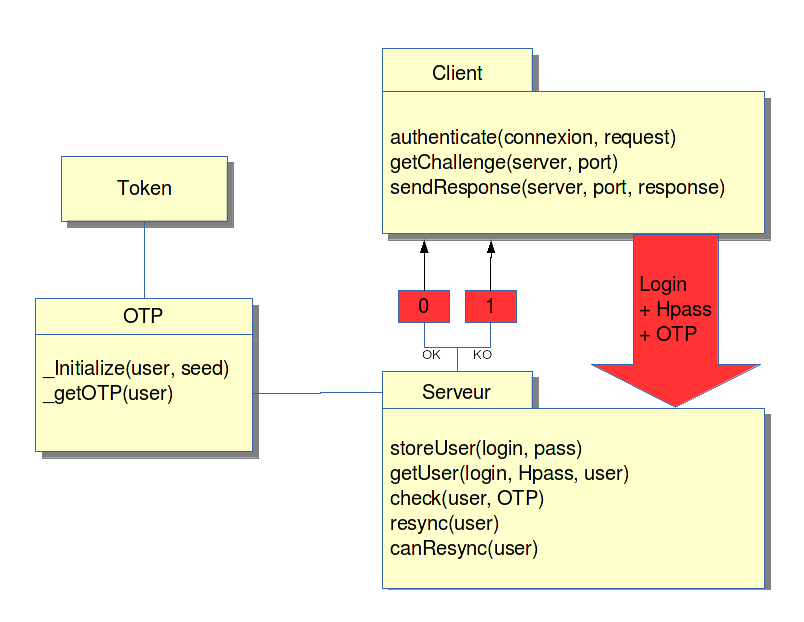
\includegraphics[width=\textwidth]{../graphics/architecture.png}
\subsection{Structure user}
\label{sub:Structure_user}
    Cette structure a pour but de pouvoir conserver l'état d'un générateur d'OTP
    pour un utilisateur. Elle sera stockée dans une base de données sur le
    serveur. Cela permet de ne charger qu'un seul module de génération de mot de
    passe en mémoire pour gérer plusieurs utilisateurs.
    \subsubsection{Champs}
    \label{ssub:Champs}
        Une structure identifiant un utilisateur pour un générateur d'OTP 
        contient les champs suivants:
        \begin{description}
            \item[login] le nom de l'utilisateur
            \item[HPass] Une empreinte du mot de passe de l'utilisateur
            \item[isLocked] indique si l'utilisateur à le droit d'essayer de
                se connecter
            \item[secret] Le secret permettant de générer n'importe quel OTP 
                valide
            \item[how] La méthode d'authentification OTP.
            \item[otparams] Un pointeur vers une structure contenant des 
                paramêtres relatifs à la méthode de génération d'OTP
        \end{description}

\subsection{Token}
    \subsubsection{Rôle}
        Afficher les mots de passe jetables pour un utilisateur donné.

    \subsubsection{Propriétés et attributs de caractérisation}
    \begin{description}
        \item[Secret] Le secret de l'utilisateur qui permet de générer les
            mots de passe jetables.
        \item[User] La structure qui contient les données de l'utilisateur.
            Stock\'ee dans la m\'emoire à long terme du support.
    \end{description}

    \subsubsection{Dépendances}
        \begin{itemize}
            \item Générateurs d'OTP.
            \item Toolkit d'interaction avec l'utilisateur.
        \end{itemize}

    \subsubsection{Langages de programmation}
    \begin{itemize}
        \item C
        \item Java Mobile (optionel)
        \item Java Card (optionel)
    \end{itemize}

    \subsubsection{Procédés de développement}
    \begin{enumerate}
        \item Développer des modules réalisants chaque algorithme de génération
            d'OTP.
        \item Développer un générateur de secrets.
        \item Permettre une interaction avec l'utilisateur.
    \end{enumerate}

    \subsubsection{Taille et complexité}
    \begin{itemize}
        \item Taille et compléxité dépendantes de l'algorithme de génération
            de mots de passe jetables
    \end{itemize}

%------------------------------------------------------------------------------
\subsection{Générateur d'OTP}
    Chaque algorithme \'etudi\'e et impl\'ement\'e (HOTP, OTPW, POTP) offrira les
    mêmes services, seul le fonctionnement interne du module differera.
    les algorithmes seront détaillés dans les dossiers associés au recherches sur 
    chaques algorithme.
    \subsubsection{Rôle}
        Générer des mots de passe jetables permettant de s'authentifier.

    \subsubsection{Services offerts}
    \begin{description}
        \item[initiate(user * utilisateur, char * seed):] Initialise
            un générateur d'OTP pour l'utilisateur.
        \item[getOTP(user * utilisateur)] Génère un OTP selon la méthode et les
            paramêtres passés.
    \end{description}

    \subsubsection{Langages de programmation}
    \begin{itemize}
        \item C
        \item Java Mobile (Optionel)
        \item Java Card (Optionel)
    \end{itemize}

    \subsubsection{Procédé de développement}
    \begin{enumerate}
        \item Développer des modules réalisants chaque algorithme de génération
            d'OTP.
    \end{enumerate}

    \subsubsection{Taille et complexité}
    \begin{itemize}
        \item Taille et compléxité dépendantes de l'algorithme de génération
            de mots de passe jetables, mais suffisamment faibles pour tenir sur
            de petites capacités mémoire et permettre un calcul 
            en t < 1s sur \verb?700MHz?.
    \end{itemize}

\subsection{Client}
    \subsubsection{Rôle}
        Permettre une authentification sur un service en demandant à
    l'utilisateur un mot de passe jetable.

    \subsubsection{Services offerts}
    \begin{description}
        \item[authenticate(connection * c, req * request):] Permet
            de s'authentifier auprès du serveur \verb?server? sur 
            le port \verb?port?, d'après la requête \verb?request?.
    \end{description}

    \subsubsection{Dépendance}
    \begin{itemize}
        \item Sockets Berkeley
    \end{itemize}

    \subsubsection{Langage de programmation}
    \begin{itemize}
        \item C
    \end{itemize}

    \subsubsection{Procédé de développement}
    \begin{enumerate}
        \item Déterminer le protocole d'échange entre le client et le
            serveur.
        \item Déterminer le contenu d'une requête.
    \end{enumerate}

    \subsubsection{Taille et complexité}
        Le client ne consiste qu'en l'envoi et la réception de données sur le
        réseau, donc la taille et la complexité sont faibles.

\subsection{Serveur}
    \subsubsection{Rôle}
    Dire si un mot de passe jetable est valide ou non pour s'authentifier sur un
    service donné.

    \subsubsection{Propriétés et attributs de caractérisation}
    \begin{description}
        \item[Port] Le port utilisé pour accéder au serveur
            d'authentification.
        \item[Adresse] L'adresse pour accéder au serveur 
            d'authentification.
    \end{description}

    \subsubsection{Services offerts}
    \begin{description}
        \item[associate(user * u, char * secret):] Associe un secret à un 
            utilisateur.
        \item[check(user * u, char * OTP):] Vérifie que l'OTP est valide pour
            l'utilisateur.
        \item[lock(user * u):] Interdit la connection pour un utilisateur.
        \item[warn(user * u):] Prévient par mail un utilisateur de son 
            verrouillage.
        \item[resynchronize(user * u):] Demande une resynchronisation pour
            un utilisateur donné.
    \end{description}

    \subsubsection{Dépendances}
    \begin{itemize}
        \item Sockets Berkeley.
        \item Générateurs d'OTP.
    \end{itemize}

    \subsubsection{Langage de programmation}
    \begin{itemize}
        \item C
    \end{itemize}

    \subsubsection{Procédés de développement}
    \begin{enumerate}
        \item Déterminer le protocole de communication entre client et serveur.
        \item Déterminer le contenu d'une requête d'authentification
        \item Utiliser les modules de génération d'OTP pour les vérifications de
        validité d'OTP.
    \end{enumerate}        

    \subsubsection{Taille et complexité}
    Probablement le composant le plus volumineux du système, puisqu'il doit être
    en mesure de supporter plusieurs requêtes simultanées ainsi que plusieurs
    protocoles de mots de passe jetables.


\subsection{Justification des choix techniques}
\subsubsection{Le langage C}
Le langage C a été choisi pour 2 raisons:
\begin{enumerate}
    \item Car il est supposé connu de tout les membres de l'équipe, au vu
        de l'enseignement reçu.
    \item Car il permet de mieux maîtriser l'aspect sécurité en évitant un
        nombre trop important de dépendances intermédiaires dont on ne peut
        garantir la sécurité.
\end{enumerate}

%-------------------------------------------------------------------------------
\subsubsection{Le langage Java}
    Le langage java sera utilis\'e sur les plateformes android
    et javacard, car bien qu'il soit possible de programmer en C
    sur android, ce n'est pas recommand\'e par \verb?Google?
    \footnote{\href{https://developer.android.com/tools/sdk/ndk/index.html}{Android NDK}}.
        
\section{Fonctionnement dynamique}
\subsection{Association/Partage du secret}
\subsubsection{Principe}
Le token et le serveur se mettent d'accord sur un secret partag\'e gr\^ace à l'utilisateur.

\subsubsection{Fonctionnement}
\begin{enumerate}
    \item partage du secret via une saisie utilisateur.
    \item Indiquer l'échec ou la réussite de l'opération
\end{enumerate}
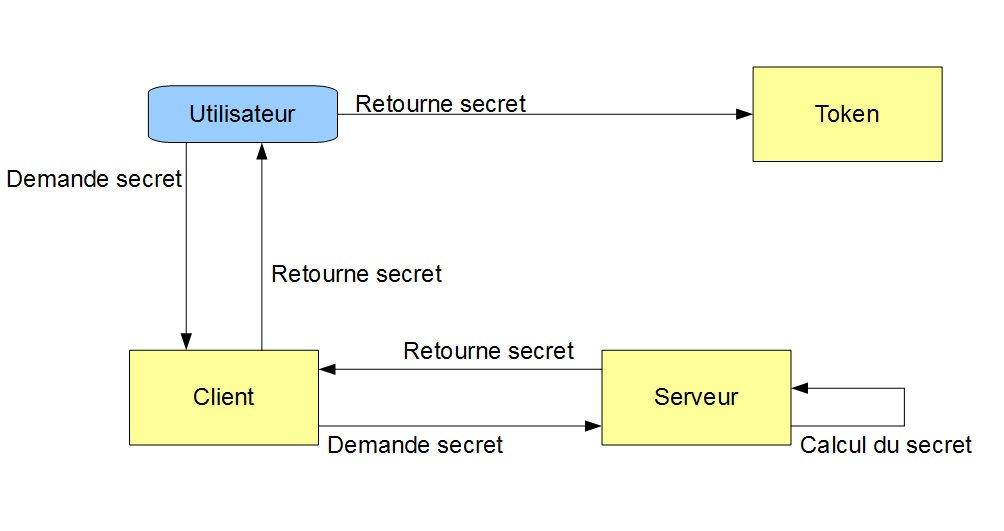
\includegraphics[width=\textwidth]{../graphics/association.jpg}

\subsection{Génération d'un mot de passe jetable}
\subsubsection{Principe}
Le token donne un mot de passe jetable à l'utilisateur.

\subsubsection{Fonctionnement}
\begin{enumerate}
    \item Calcul d'un mot de passe jetable à partir du secret 
        initial
\end{enumerate}
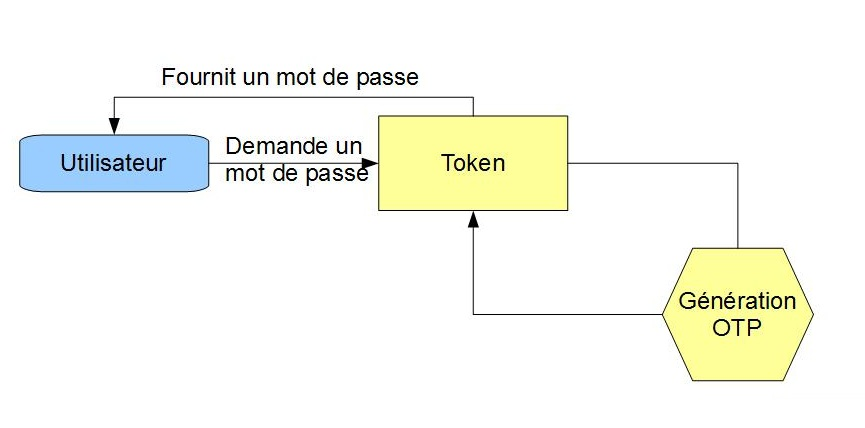
\includegraphics[width=\textwidth]{../graphics/generation.jpg}

\subsection{Authentification}
\subsubsection{Principe}
On entre le mot de passe généré par le token dans le client qui demandera une
vérification au serveur.

\subsubsection{Fonctionnement}
\begin{enumerate}
    \item L'utilisateur entre le mot de passe
    \item Le client demande au serveur de vérifier la validité du
        mot de passe
    \item Le client répond:
        \begin{description}
            \item[OK] Si le serveur accepte le mot de passe
            \item[KO] Si le serveur refuse le mot de passe
        \end{description}
\end{enumerate}
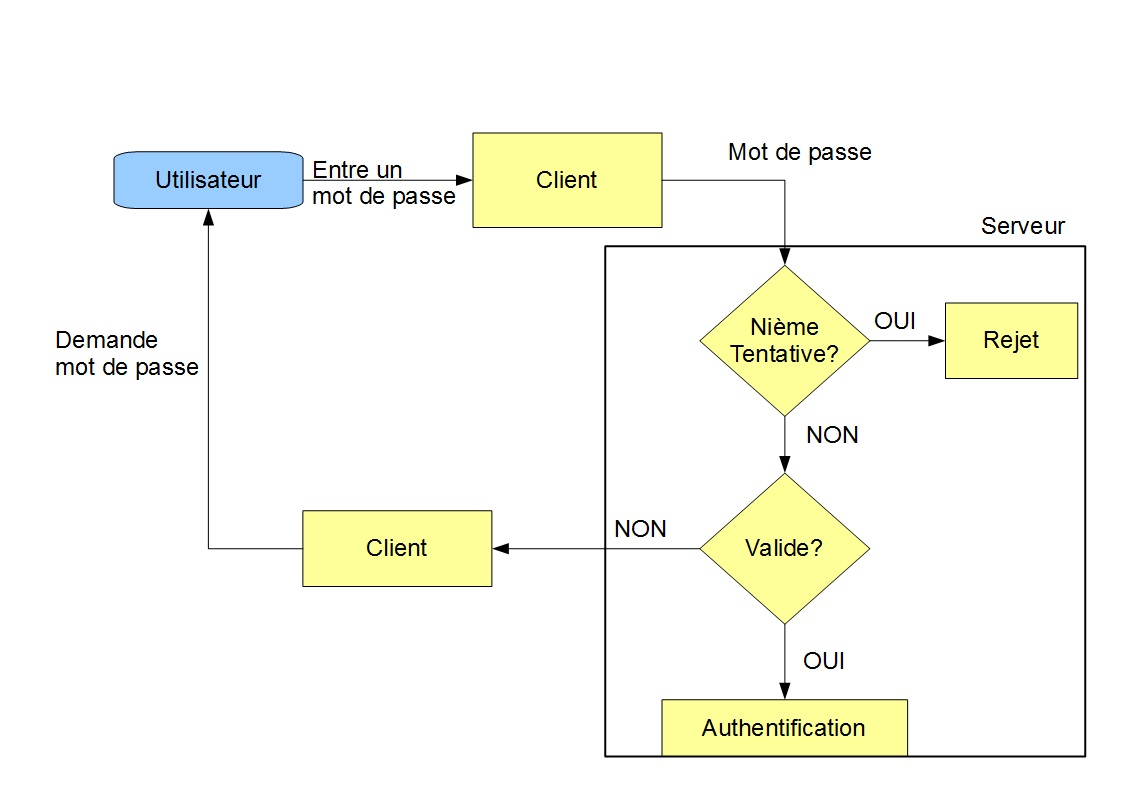
\includegraphics[width=\textwidth]{../graphics/authentification.jpg}

\subsection{Resynchronisation}
\subsubsection{Principe}
Le serveur et le token se resynchronisent pour être d'accord sur la suite des
mots de passe jetables générés.

\subsubsection{Fonctionnement}
\begin{enumerate}
    \item L'utilisateur ou le serveur font une demande de resynchronisation
    \item Le serveur et le token se mettent d'accord sur l'état de la suite des
    mots de passe jetables.
\end{enumerate}
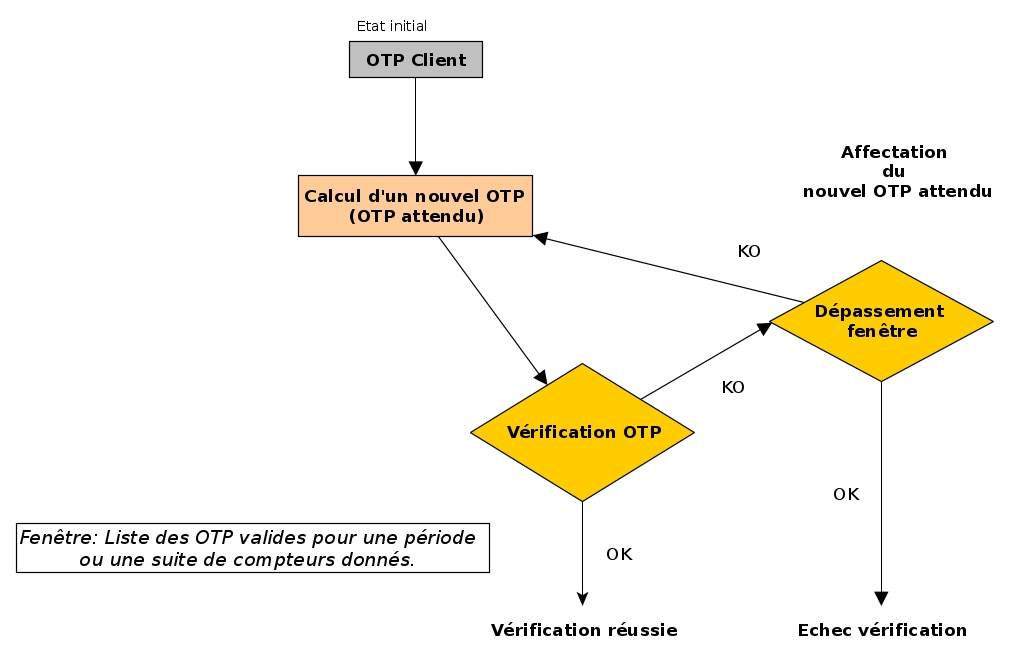
\includegraphics[width=\textwidth]{../graphics/resynchronisation.jpg}
\end{document}
